\chapter{Trabalhos Relacionados}

É inerente ao paradigma SDN a centralização lógica da rede em um único controlador. Entretanto, devido à variedade de serviços prestados e ao possível crescimento da infraestrutura de redes, projetar um plano de controle distribuído tornou-se uma opção a ser analisada para evitar o gargalo em um único controlador. O OpenFlow, apesar de ser o padrão de interface para comunicação entre plano de dados e controle, não possui uma definição para comunicação entre controladores para o caso de um plano de controle distribuído. Esta seção apresenta alguns trabalhos com possíveis soluções para o gerenciamento de controladores distribuídos..

\section{HyperFlow}

O trabalho de \citeonline{hiperflow} foi o primeiro a propor uma aplicação para o plano de controle distribuído: o HiperFlow. Essa solução foi implementada como uma aplicação específica no controlador NOX, dessa forma, para utilizá-lo de forma distribuída deve-se instanciar todos os controladores dentro da mesma rede OpenFlow de forma que  cada instância controle um certo número de \emph{switches} e cada \emph{switch} seja controlado por somente um controlador, como ilustra a Figura \ref{hyperflow}.
\par O funcionamento do Hyperflow é baseado em eventos, assim, a aplicação em uma instância é responsável por capturar todos os eventos ocorridos em sua área e em seguida divulgá-los aos outros controladores utilizando o paradigma publicação/assinatura. Para realizar essa divulgação o HyperFlow utiliza o WheelFS\cite{Stribling}, um sistema de arquivos projetado especificamente para armazenamento de arquivos em sistemas distribuídos. Dessa forma, o HyperFlow somente define um diretório como canal de comunicação dos eventos,checando-o periodicamente por possíveis mudanças, e estes serão divulgados pelo WheelFs através de arquivos neste mesmo diretório. 

\pagebreak
\begin{figure}[!h]
	\caption{ Arquitetura do HyperFlow}
  \centering
  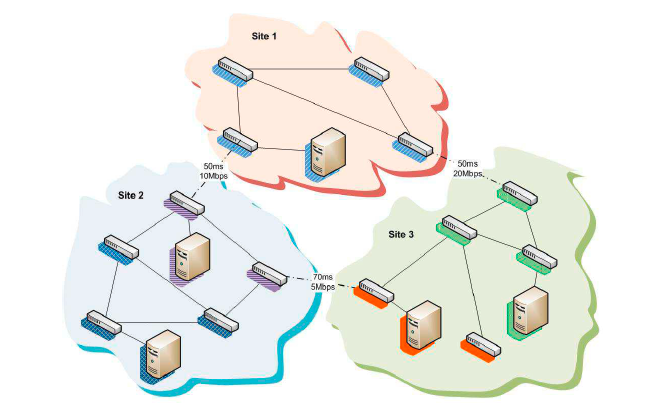
\includegraphics[scale=1]{Imagens/hiperflow.PNG} 
 
  \legend{Fonte: \citeonline{hiperflow}}
  \label{hyperflow}
\end{figure}

\par A partir dessa arquitetura todas as solicitações podem ser atendidas localmente pelos controladores, reduzindo o tráfego entre as áreas e ainda mantendo a visão global da rede. Além disso, caso algum controlador responsável por uma área falhe, outro controlador pode e irá assumir sua função, já que todos as informações necessárias estarão nos arquivos divulgados. O problema citado dessa arquitetura é justamente a necessidade de se implementar diversas instâncias do HyperFlow em cada controlador NOX, implicando em alterar o código no núcleo do controlador para interceptar comandos e serializar eventos.

\section{Onix}

A proposta de \citeonline{onix} consiste no Onix, uma aplicação para controladores distribuídos que se difere de outros trabalhos por expor uma interface mais genérica, tendo como alvo ambientes diversos como redes WAN, nuvens públicas e centros de dados corporativos.Além disso, provê meios para distribuições flexíveis permitindo que os \emph{designers} de aplicações implementem aplicações de controle sem reinventar mecanismos de distribuições e mantendo requisitos de escalabilidade e performance. De acordo com a Figura \ref{onix}, existem 4 componentes em uma rede controlada pelo Onix:

\begin{itemize}
    \item Infraestrutura física: Inclui \emph{switches} e roteadores e outras entidades físicas que permitam que Onix leia e escreva o estado que controla o comportamento do elemento, como em uma espécie de tabela de encaminhamento.
    \item Infraestrutura de conexão: Corresponde à comunicação entre o Onix e a infraestrutura física. Esse canal de controle pode ser implementando tanto na banda(tráfego de controle compartilha a mesma conexão com o tráfego de dados), como fora da banda(tráfego de controle e dados utilizam conexões separadas) e deve fornecer ainda comunicação bidirecional.
    \item Onix: Sistema distribuído que é executado em um cluster composto de um ou mais sevidores físicos, onde cada um pode executar múltiplas instâncias do Onix. O Onix é responsável por fornecer acesso lógico de controle à rede(em ações como escrever e ler o estado da rede) e disseminar o estado da rede para outras instâncias dentro do cluster.
    \item Lógica de controle: A lógica de controle da rede é implementada no topo da interface do Onix. Essa lógica determina o comportamento desejado da rede. O Onix somente fornece os meios necessários para acessar o estado apropriado da rede.
\end{itemize}


\begin{figure}[!h]
	\caption{ Arquitetura do Onix}
  \centering
  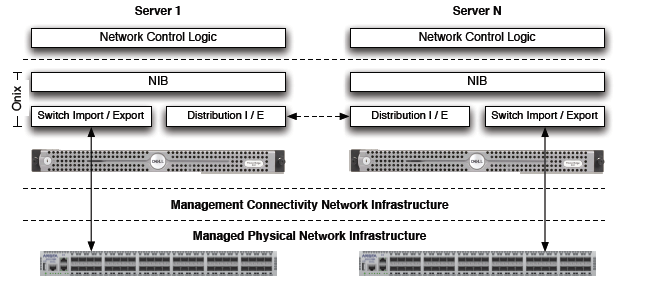
\includegraphics[scale=1]{Imagens/onix.png} 
 
  \legend{Fonte: \citeonline{onix}}
  \label{onix}
\end{figure}

O Onix utiliza um modelo de dados chamado \emph{Network Information Base} (NIB). Este modelo faz o controle do estado da rede através de uma estrutura de dados que armazena um grafo das entidades da topologia da rede. É através da replicação e distribuição desse modelo NIB que o Onix consegue prover a escalabilidade. Para que ocorra a sincronização de dados sem falha entre os processos distribuídos, o Onix utiliza a API Apache Zookeeper, possibilitando que o mesmo mantenha, por exemplo, informações de configuração, nomeação de servidores e provendo serviços para grupos específicos da rede. Apesar de sua contribuição relevante, tendo se baseado no contolador NOX e no Apache ZooKeeper, o Onix foi desenvolvido em código fechado, impossibilitando a integração e o desenvolvimento de novas aplicações.
\pagebreak
\section{DISCO - \emph{DIstributed SDN COntrol Plane} }

O trabalho de \citeonline{disco} apresenta outra possibilidade para integração de controladores DISCO. A implementação se baseia nos controladores Floodlight, cada qual com seu domínio da rede. Por sua vez estes se comunicam para manter uma visão global da rede utilizando uma interface \emph{East/West} através do \emph{Advanced Message Queuing Protocol} (AMQP)\cite{amqp}. O OpenFlow se mantém como interface \emph{SouthBound} para comunicação com a camada de dados da rede.
    O conceito utilizado pelo DISCO é que cada controlador Floodlight possui um agente configurado que permite trocar informações sobre os domínios adjacentes utilizando o AMQP. Essa API é composta de um módulo que identifica os controladores vizinhos, possibilitando a troca de mensagens. Entre os agentes descritos temos:
    
    \begin{itemize}
        \item O agente de conectividade, responsável pelo peering;
        \item O agente de monitoramento, responsável por buscar informações sobre largura de banda e latência;
        \item O agente de acessibilidade, responsável por avisar caso apareça um novo host no domínio;
        \item O agente de reserva, que utiliza o \emph{Resource reServation Protocol} (RSVP) para
        fornecer recursos fim-a-fim;
    \end{itemize}

O maior desafio relacionado ao DISCO é que este utiliza módulos exlusivos para o controlador Floodlight, tornando a aplicação dependente destes.

\section{OrchFlow}

O trabalho de \citeonline{frate} surgiu em meio aos desafios verificados em trabalhos anteriores. Ele sugere a ferramenta OrchFlow como software orquestrador para redes SDN baseadas no OpenFlow. 
  A Figura \ref{orchflow} ilustra a arquitetura do Orchflow. Ele atua como um agente integrador entre as aplicações disponíveis na rede e também entre os diversos controladores que gerenciam subdomínios sob um mesmo domínio administrativo. Na base da arquitetura temos os \emph{switches}, que formam a infraestrutura da camada de dados; e para cada conjunto de \emph{switches} temos um um subdomínio da rede que é controlado por um controlador SDN através do OpenFlow. Cada controlador está conectado ao OrchFlow através de uma interface central, que independe da linguagem de programação do controlador. Além disso, o OrchFlow possibilita a comunicação entre diferentes aplicações através da interface \emph{NorthBound}, recebendo solicitações específicas de serviços pré-determinados pelo OrchFlow. Essa integração entre aplicações e controladores só é possível porque utiliza-se uma Interface \emph{Representational State Transfer} (REST), que aplica regras estabelecidas para a aplicação solicitante e entrega para o controlador adequado, conforme seu subdomínio.O OrchFlow ainda fornece três modos de atuação: o Proativo, o Reativo e o Híbrido, que dizem respeito a forma de gerenciamento dos fluxos entre os \emph{switches}.
  
\begin{figure}[!h]
	\caption{ Arquitetura do OrchFlow}
  \centering
  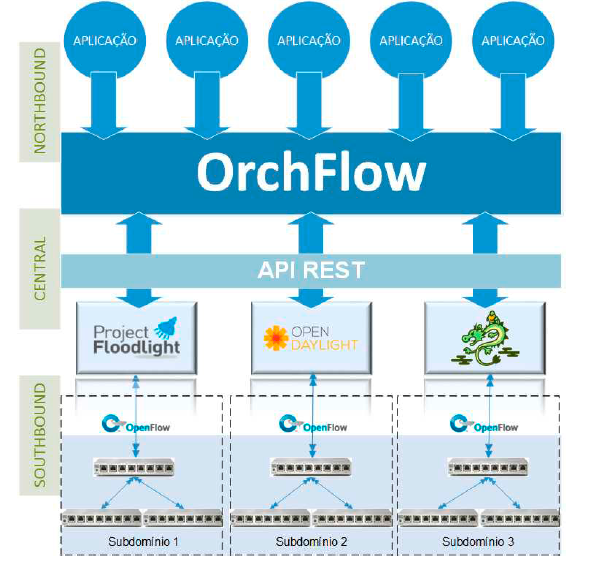
\includegraphics[scale= 0.8] {Imagens/orchflow.PNG} 
 
  \legend{Fonte: \citeonline{frate}}
  \label{orchflow}
\end{figure}

Com relação a sua implementação, a linguagem java foi escolhida para a implementação do OrchFlow. Além disso, para armazenamento dos dados, utiliza-se o banco de dados Neo4j \cite{neo}, um banco de dados orientado a grafos também baseado em Java, que oferece persistência, alto desempenho, escalabilidade e com boa documentação. 
\par A possibilidade da escalabilidade para gerenciar qualquer número de controladores implementados em qualquer linguagem, sob uma topologia hierárquica ou não e ainda com uma interface WEB torna o OrchFlow um orquestrador diferenciado, entretanto, seus testes ocorreram somente com os controladores Ryu e FLoodlight, sendo necessário mais testes para otimização de códigos com outros tipos de controladores, bem como com outros tipos de aplicações.












